

\documentclass[11pt,fleqn]{book} % Default font size and left-justified equations

%%%%%%%%%%%%%%%%%%%%%%%%%%%%%%%%%%%%%%%%%
% The Legrand Orange Book
% Structural Definitions File
% Version 2.0 (9/2/15)
%
% Original author:
% Mathias Legrand (legrand.mathias@gmail.com) with modifications by:
% Vel (vel@latextemplates.com)
% 
% This file has been downloaded from:
% http://www.LaTeXTemplates.com
%
% License:
% CC BY-NC-SA 3.0 (http://creativecommons.org/licenses/by-nc-sa/3.0/)
%
%%%%%%%%%%%%%%%%%%%%%%%%%%%%%%%%%%%%%%%%%

%----------------------------------------------------------------------------------------
%	VARIOUS REQUIRED PACKAGES AND CONFIGURATIONS
%----------------------------------------------------------------------------------------

\usepackage[top=3cm,bottom=3cm,left=5.5cm,right=3cm,headsep=10pt,letterpaper,asymmetric]{geometry} % Page margins
% Could use 6cm margin on left 

\usepackage{graphicx} % Required for including pictures
\graphicspath{{Pictures/}} % Specifies the directory where pictures are stored

\usepackage{lipsum} % Inserts dummy text

\usepackage{tikz} % Required for drawing custom shapes

\usepackage[english]{babel} % English language/hyphenation

\usepackage{enumitem} % Customize lists
\setlist{noitemsep} % Reduce spacing between bullet points and numbered lists

\usepackage{booktabs} % Required for nicer horizontal rules in tables

\usepackage{xcolor} % Required for specifying colors by name
%\definecolor{rust}{RGB}{243,102,25} % Define the orange color used for highlighting throughout the book
\definecolor{rust}{RGB}{153, 0, 0} % Define alternate red color

\usepackage{pdftexcmds}



%----------------------------------------------------------------------------------------
%	FONTS
%----------------------------------------------------------------------------------------

\usepackage{avant} % Use the Avantgarde font for headings
%\usepackage{times} % Use the Times font for headings
\usepackage{mathptmx} % Use the Adobe Times Roman as the default text font together with math symbols from the Sym­bol, Chancery and Com­puter Modern fonts

\usepackage{microtype} % Slightly tweak font spacing for aesthetics
\usepackage[utf8]{inputenc} % Required for including letters with accents
\usepackage[T1]{fontenc} % Use 8-bit encoding that has 256 glyphs
\usepackage{relsize} % Allow relative font sizing
\renewcommand\RSlargest{100pt} 
%----------------------------------------------------------------------------------------
%	BIBLIOGRAPHY AND INDEX
%----------------------------------------------------------------------------------------

\usepackage[style=alphabetic,citestyle=numeric,sorting=nyt,sortcites=true,autopunct=true,babel=hyphen,hyperref=true,abbreviate=false,backref=true,backend=biber]{biblatex}
\addbibresource{bibliography.bib} % BibTeX bibliography file
\defbibheading{bibempty}{}

\usepackage{calc} % For simpler calculation - used for spacing the index letter headings correctly
\usepackage{makeidx} % Required to make an index
\makeindex % Tells LaTeX to create the files required for indexing

%----------------------------------------------------------------------------------------
%	MAIN TABLE OF CONTENTS
%----------------------------------------------------------------------------------------

\usepackage{titletoc} % Required for manipulating the table of contents

\contentsmargin{0cm} % Removes the default margin

% Part text styling
\titlecontents{part}[0cm]
{\addvspace{20pt}\centering\large\bfseries}
{}
{}
{}

% Chapter text styling
\titlecontents{chapter}[1.25cm] % Indentation
{\addvspace{12pt}\large\sffamily\bfseries} % Spacing and font options for chapters
{\color{rust!60}\contentslabel[\Large\thecontentslabel]{1.25cm}\color{rust}} % Chapter number
{\color{rust}}  
{\color{rust!60}\normalsize\;\titlerule*[.5pc]{.}\;\thecontentspage} % Page number

% Section text styling
\titlecontents{section}[1.25cm] % Indentation
{\addvspace{3pt}\sffamily\bfseries} % Spacing and font options for sections
{\contentslabel[\thecontentslabel]{1.25cm}} % Section number
{}
{\hfill\color{black}\thecontentspage} % Page number
[]

% Subsection text styling
\titlecontents{subsection}[1.25cm] % Indentation
{\addvspace{1pt}\sffamily\small} % Spacing and font options for subsections
{\contentslabel[\thecontentslabel]{1.25cm}} % Subsection number
{}
{\ \titlerule*[.5pc]{.}\;\thecontentspage} % Page number
[]

% List of figures
\titlecontents{figure}[0em]
{\addvspace{-5pt}\sffamily}
{\thecontentslabel\hspace*{1em}}
{}
{\ \titlerule*[.5pc]{.}\;\thecontentspage}
[]

% List of tables
\titlecontents{table}[0em]
{\addvspace{-5pt}\sffamily}
{\thecontentslabel\hspace*{1em}}
{}
{\ \titlerule*[.5pc]{.}\;\thecontentspage}
[]

%----------------------------------------------------------------------------------------
%	MINI TABLE OF CONTENTS IN PART HEADS
%----------------------------------------------------------------------------------------

% Chapter text styling
\titlecontents{lchapter}[0em] % Indenting
{\addvspace{15pt}\large\sffamily\bfseries} % Spacing and font options for chapters
{\color{rust}\contentslabel[\Large\thecontentslabel]{1.25cm}\color{rust}} % Chapter number
{}  
{\color{rust}\normalsize\sffamily\bfseries\;\titlerule*[.5pc]{.}\;\thecontentspage} % Page number

% Section text styling
\titlecontents{lsection}[0em] % Indenting
{\sffamily\small} % Spacing and font options for sections
{\contentslabel[\thecontentslabel]{1.25cm}} % Section number
{}
{}

% Subsection text styling
\titlecontents{lsubsection}[.5em] % Indentation
{\normalfont\footnotesize\sffamily} % Font settings
{}
{}
{}

%----------------------------------------------------------------------------------------
%	PAGE HEADERS
%----------------------------------------------------------------------------------------

\usepackage{fancyhdr} % Required for header and footer configuration

\pagestyle{fancy}
\renewcommand{\chaptermark}[1]{\markboth{\sffamily\normalsize\bfseries\chaptername\ \thechapter.\ #1}{}} % Chapter text font settings
\renewcommand{\sectionmark}[1]{\markright{\sffamily\normalsize\thesection\hspace{5pt}#1}{}} % Section text font settings
\fancyhf{} \fancyhead[LE,RO]{\sffamily\normalsize\thepage} % Font setting for the page number in the header
\fancyhead[LO]{\rightmark} % Print the nearest section name on the left side of odd pages
\fancyhead[RE]{\leftmark} % Print the current chapter name on the right side of even pages
\renewcommand{\headrulewidth}{0.5pt} % Width of the rule under the header
\addtolength{\headheight}{2.5pt} % Increase the spacing around the header slightly
\renewcommand{\footrulewidth}{0pt} % Removes the rule in the footer
\fancypagestyle{plain}{\fancyhead{}\renewcommand{\headrulewidth}{0pt}} % Style for when a plain pagestyle is specified

% Removes the header from odd empty pages at the end of chapters
\makeatletter
\renewcommand{\cleardoublepage}{
\clearpage\ifodd\c@page\else
\hbox{}
\vspace*{\fill}
\thispagestyle{empty}
\newpage
\fi}

%----------------------------------------------------------------------------------------
%	THEOREM STYLES
%----------------------------------------------------------------------------------------

\usepackage{amsmath,amsfonts,amssymb,amsthm} % For math equations, theorems, symbols, etc

\newcommand{\intoo}[2]{\mathopen{]}#1\,;#2\mathclose{[}}
\newcommand{\ud}{\mathop{\mathrm{{}d}}\mathopen{}}
\newcommand{\intff}[2]{\mathopen{[}#1\,;#2\mathclose{]}}
\newtheorem{notation}{Notation}[chapter]

% Boxed/framed environments
\newtheoremstyle{rustnumbox}% % Theorem style name
{0pt}% Space above
{0pt}% Space below
{\normalfont}% % Body font
{}% Indent amount
{\small\bf\sffamily\color{rust}}% % Theorem head font
{\;}% Punctuation after theorem head
{0.25em}% Space after theorem head
{\small\sffamily\color{rust}\thmname{#1}\nobreakspace\thmnumber{\@ifnotempty{#1}{}\@upn{#2}}% Theorem text (e.g. Theorem 2.1)
\thmnote{\nobreakspace\the\thm@notefont\sffamily\bfseries\color{black}---\nobreakspace#3.}} % Optional theorem note
\renewcommand{\qedsymbol}{$\blacksquare$}% Optional qed square

\newtheoremstyle{blacknumex}% Theorem style name
{5pt}% Space above
{5pt}% Space below
{\normalfont}% Body font
{} % Indent amount
{\small\bf\sffamily}% Theorem head font
{\;}% Punctuation after theorem head
{0.25em}% Space after theorem head
{\small\sffamily{\tiny\ensuremath{\blacksquare}}\nobreakspace\thmname{#1}\nobreakspace\thmnumber{\@ifnotempty{#1}{}\@upn{#2}}% Theorem text (e.g. Theorem 2.1)
\thmnote{\nobreakspace\the\thm@notefont\sffamily\bfseries---\nobreakspace#3.}}% Optional theorem note

\newtheoremstyle{blacknumbox} % Theorem style name
{0pt}% Space above
{0pt}% Space below
{\normalfont}% Body font
{}% Indent amount
{\small\bf\sffamily}% Theorem head font
{\;}% Punctuation after theorem head
{0.25em}% Space after theorem head
{\small\sffamily\thmname{#1}\nobreakspace\thmnumber{\@ifnotempty{#1}{}\@upn{#2}}% Theorem text (e.g. Theorem 2.1)
\thmnote{\nobreakspace\the\thm@notefont\sffamily\bfseries---\nobreakspace#3.}}% Optional theorem note

% Non-boxed/non-framed environments
\newtheoremstyle{rustnum}% % Theorem style name
{5pt}% Space above
{5pt}% Space below
{\normalfont}% % Body font
{}% Indent amount
{\small\bf\sffamily\color{rust}}% % Theorem head font
{\;}% Punctuation after theorem head
{0.25em}% Space after theorem head
{\small\sffamily\color{rust}\thmname{#1}\nobreakspace\thmnumber{\@ifnotempty{#1}{}\@upn{#2}}% Theorem text (e.g. Theorem 2.1)
\thmnote{\nobreakspace\the\thm@notefont\sffamily\bfseries\color{black}---\nobreakspace#3.}} % Optional theorem note
\renewcommand{\qedsymbol}{$\blacksquare$}% Optional qed square
\makeatother

% Defines the theorem text style for each type of theorem to one of the three styles above
\newcounter{dummy} 
\numberwithin{dummy}{section}
\theoremstyle{rustnumbox}
\newtheorem{theoremeT}[dummy]{Theorem}
\newtheorem{assignment}{Assignment}[chapter]

\newtheorem{exerciseT}{Exercise}[chapter]
\theoremstyle{blacknumex}
\newtheorem{exampleT}{Example}[chapter]
\theoremstyle{blacknumbox}
\newtheorem{vocabulary}{Vocabulary}[chapter]
\newtheorem{definitionT}{Definition}[section]
\newtheorem{corollaryT}[dummy]{Corollary}
\theoremstyle{rustnum}
\newtheorem{proposition}[dummy]{Proposition}

%----------------------------------------------------------------------------------------
%	DEFINITION OF COLORED BOXES
%----------------------------------------------------------------------------------------

\RequirePackage[framemethod=default]{mdframed} % Required for creating the theorem, definition, exercise and corollary boxes

% Theorem box
\newmdenv[skipabove=7pt,
skipbelow=7pt,
backgroundcolor=black!5,
linecolor=rust,
innerleftmargin=5pt,
innerrightmargin=5pt,
innertopmargin=5pt,
leftmargin=0cm,
rightmargin=0cm,
innerbottommargin=5pt]{tBox}

% Exercise box	  
\newmdenv[skipabove=7pt,
skipbelow=7pt,
rightline=false,
leftline=true,
topline=false,
bottomline=false,
backgroundcolor=rust!10,
linecolor=rust,
innerleftmargin=5pt,
innerrightmargin=5pt,
innertopmargin=5pt,
innerbottommargin=5pt,
leftmargin=0cm,
rightmargin=0cm,
linewidth=4pt]{eBox}	

% Definition box
\newmdenv[skipabove=7pt,
skipbelow=7pt,
rightline=false,
leftline=true,
topline=false,
bottomline=false,
linecolor=rust,
innerleftmargin=5pt,
innerrightmargin=5pt,
innertopmargin=0pt,
leftmargin=0cm,
rightmargin=0cm,
linewidth=4pt,
innerbottommargin=0pt]{dBox}	

% Corollary box
\newmdenv[skipabove=7pt,
skipbelow=7pt,
rightline=false,
leftline=true,
topline=false,
bottomline=false,
linecolor=gray,
backgroundcolor=black!5,
innerleftmargin=5pt,
innerrightmargin=5pt,
innertopmargin=5pt,
leftmargin=0cm,
rightmargin=0cm,
linewidth=4pt,
innerbottommargin=5pt]{cBox}

% Creates an environment for each type of theorem and assigns it a theorem text style from the "Theorem Styles" section above and a colored box from above
\newenvironment{theorem}{\begin{tBox}\begin{theoremeT}}{\end{theoremeT}\end{tBox}}
\newenvironment{exercise}{\begin{eBox}\begin{exerciseT}}{\hfill{\color{rust}\tiny\ensuremath{\blacksquare}}\end{exerciseT}\end{eBox}}				  
\newenvironment{definition}{\begin{dBox}\begin{definitionT}}{\end{definitionT}\end{dBox}}	
\newenvironment{example}{\begin{exampleT}}{\hfill{\tiny\ensuremath{\blacksquare}}\end{exampleT}}		
\newenvironment{corollary}{\begin{cBox}\begin{corollaryT}}{\end{corollaryT}\end{cBox}}	

%----------------------------------------------------------------------------------------
%	WARNING ENVIRONMENT
%----------------------------------------------------------------------------------------

\newenvironment{warning}{\par\vspace{10pt}\small % Vertical white space above the remark and smaller font size
	\begin{list}{}{
			\leftmargin=35pt % Indentation on the left
			\rightmargin=25pt}\item\ignorespaces % Indentation on the right
		\makebox[-2.5pt]{\begin{tikzpicture}[overlay]
			\node[draw=rust!60,line width=1pt,circle,fill=rust!25,font=\sffamily\bfseries,inner sep=2pt,outer sep=0pt] at (-15pt,0pt){\textcolor{rust}{\textbf{!}}};\end{tikzpicture}} 
		\advance\baselineskip -1pt}{\end{list}\vskip5pt} % Tighter line spacing and white space after remark

%----------------------------------------------------------------------------------------
%	REMARK ENVIRONMENT
%----------------------------------------------------------------------------------------

\newenvironment{remark}{\par\vspace{10pt}\small % Vertical white space above the remark and smaller font size
\begin{list}{}{
\leftmargin=35pt % Indentation on the left
\rightmargin=25pt}\item\ignorespaces % Indentation on the right
\makebox[-2.5pt]{\begin{tikzpicture}[overlay]
\node[draw=rust!60,line width=1pt,circle,fill=rust!25,font=\sffamily\bfseries,inner sep=2pt,outer sep=0pt] at (-15pt,0pt){\textcolor{rust}{R}};\end{tikzpicture}} % Orange R in a circle
\advance\baselineskip -1pt}{\end{list}\vskip5pt} % Tighter line spacing and white space after remark

%----------------------------------------------------------------------------------------
%	SECTION NUMBERING IN THE MARGIN
%----------------------------------------------------------------------------------------

\makeatletter

% just bottom line
%\newmdenv[topline=false,leftline=false,rightline=false]{test123}

%\newmdenv[
%rightline=false, leftline=false, topline=false, bottomline=true,
%linecolor=rust, linewidth=4pt
%]{sectionUnderline}

% Adjusts all numbering for sections and subsections
\renewcommand{\@seccntformat}[1]{  
    \ifnum\pdf@strcmp{#1}{section}=\z@ 
    
    %\llap{\colorbox{gray!15}{\makebox[3.25cm][r]{\textcolor{gray}{\textsc{\@nameuse{secTypeName}}\hspace{0.5em}\relsize{1.25}\textcolor{rust}{\csname the#1\endcsname}}}}\hspace{.5em}}
    \llap{
        %\begin{sectionUnderline}
            \makebox[3.25cm][r]{\textcolor{gray}{\textsc{\@nameuse{secTypeName}}\hspace{0.5em}\relsize{1.25}\textcolor{rust}{\csname the#1\endcsname}}}
            \textcolor{rust}{\hspace{-3.25cm}\rule[-.2cm]{3.13cm}{2pt}}
        %\end{sectionUnderline}
        \hspace{.5em}
    }
    \else
    \llap{\textcolor{rust}{\csname the#1\endcsname}\hspace{1em}}%
    \fi 
   % \llap{\textcolor{rust}{\csname the#1\endcsname}\hspace{1em}}
}  % hspace controls spacing of section number to section name    


\newcommand{\setSectionType}[1]{
    \@namedef{secTypeName}{#1}
}
        
\renewcommand{\section}{\@startsection{section}{1}{-8pt}
{-5ex \@plus -1ex \@minus -.2ex}
{2.0ex \@plus.2ex }
{\normalfont\large\sffamily\bfseries}}


\renewcommand{\subsection}{\@startsection {subsection}{2}{-3pt}
{-3ex \@plus -0.1ex \@minus -.4ex}
{0.5ex \@plus.2ex }
{\normalfont\sffamily\bfseries}}
\renewcommand{\subsubsection}{\@startsection {subsubsection}{3}{\z@}
{-2ex \@plus -0.1ex \@minus -.2ex}
{.2ex \@plus.2ex }
{\normalfont\small\sffamily\bfseries}}                        
\renewcommand\paragraph{\@startsection{paragraph}{4}{\z@}
{-2ex \@plus-.2ex \@minus .2ex}
{.1ex}
{\normalfont\small\sffamily\bfseries}}

%----------------------------------------------------------------------------------------
%	PART HEADINGS
%----------------------------------------------------------------------------------------

% numbered part in the table of contents
\newcommand{\@mypartnumtocformat}[2]{%
\setlength\fboxsep{0pt}%
\noindent\colorbox{rust!20}{\strut\parbox[c][.7cm]{\ecart}{\color{rust!70}\Large\sffamily\bfseries\centering#1}}\hskip\esp\colorbox{rust!40}{\strut\parbox[c][.7cm]{\linewidth-\ecart-\esp}{\Large\sffamily\centering#2}}}%
%%%%%%%%%%%%%%%%%%%%%%%%%%%%%%%%%%
% unnumbered part in the table of contents
\newcommand{\@myparttocformat}[1]{%
\setlength\fboxsep{0pt}%
\noindent\colorbox{rust!40}{\strut\parbox[c][.7cm]{\linewidth}{\Large\sffamily\centering#1}}}%
%%%%%%%%%%%%%%%%%%%%%%%%%%%%%%%%%%
\newlength\esp
\setlength\esp{4pt}
\newlength\ecart
\setlength\ecart{1.2cm-\esp}
\newcommand{\thepartimage}{}%
\newcommand{\partimage}[1]{\renewcommand{\thepartimage}{#1}}%
\def\@part[#1]#2{%
\ifnum \c@secnumdepth >-2\relax%
\refstepcounter{part}%
\addcontentsline{toc}{part}{\texorpdfstring{\protect\@mypartnumtocformat{\thepart}{#1}}{\partname~\thepart\ ---\ #1}}
\else%
\addcontentsline{toc}{part}{\texorpdfstring{\protect\@myparttocformat{#1}}{#1}}%
\fi%
\startcontents%
\markboth{}{}%
{\thispagestyle{empty}%
\begin{tikzpicture}[remember picture,overlay]%
\node at (current page.north west){\begin{tikzpicture}[remember picture,overlay]%	
\node[anchor=north] at (4cm,-3.25cm){\color{rust!60}\fontsize{220}{100}\sffamily\bfseries\@Roman\c@part}; 
\node[anchor=south east] at (\paperwidth-1cm,-\paperheight+1cm){\parbox[t][][t]{8.5cm}{
\printcontents{l}{0}{\setcounter{tocdepth}{1}}%
}};
\node[anchor=north east] at (\paperwidth-1.5cm,-3.25cm){\parbox[t][][t]{15cm}{\strut\raggedleft\color{black!40}\fontsize{30}{30}\sffamily\bfseries#2}};
\end{tikzpicture}};
\end{tikzpicture}}%
\@endpart}
\def\@spart#1{%
\startcontents%
\phantomsection
{\thispagestyle{empty}%
\begin{tikzpicture}[remember picture,overlay]%
\node at (current page.north west){\begin{tikzpicture}[remember picture,overlay]%	
\fill[rust!20](0cm,0cm) rectangle (\paperwidth,-\paperheight);
\node[anchor=north east] at (\paperwidth-1.5cm,-3.25cm){\parbox[t][][t]{15cm}{\strut\raggedleft\color{white}\fontsize{30}{30}\sffamily\bfseries#1}};
\end{tikzpicture}};
\end{tikzpicture}}
\addcontentsline{toc}{part}{\texorpdfstring{%
\setlength\fboxsep{0pt}%
\noindent\protect\colorbox{rust!40}{\strut\protect\parbox[c][.7cm]{\linewidth}{\Large\sffamily\protect\centering #1\quad\mbox{}}}}{#1}}%
\@endpart}
\def\@endpart{\vfil\newpage
\if@twoside
\if@openright
\null
\thispagestyle{empty}%
\newpage
\fi
\fi
\if@tempswa
\twocolumn
\fi}

%----------------------------------------------------------------------------------------
%	CHAPTER HEADINGS
%----------------------------------------------------------------------------------------

% A switch to conditionally include a picture, implemented by  Christian Hupfer
\newif\ifusechapterimage
\usechapterimagetrue
\newcommand{\thechapterimage}{}%
\newcommand{\chapterimage}[1]{\ifusechapterimage\renewcommand{\thechapterimage}{#1}\fi}%
\def\@makechapterhead#1{%
{\parindent \z@ \raggedright \normalfont
\ifnum \c@secnumdepth >\m@ne
\if@mainmatter
\begin{tikzpicture}[remember picture,overlay]
\node at (current page.north west)
{\begin{tikzpicture}[remember picture,overlay]
\node[anchor=north west,inner sep=0pt] at (0,0) {\ifusechapterimage\includegraphics[width=\paperwidth]{\thechapterimage}\fi};
%\draw[anchor=west] (\Gm@lmargin,-9cm) node [line width=2pt,rounded corners=15pt,draw=rust,fill=white,fill opacity=0.5,inner sep=15pt]{\strut\makebox[22cm]{}};

%%%%% Chapter text sizing
%\draw[anchor=west] (\Gm@lmargin-1.3cm,-4cm) node [line width=2pt,rounded corners=15pt,draw=rust,fill=white,fill opacity=0.75,inner sep=15pt]{\strut\makebox[22cm]{}};

%\draw[anchor=west] (\Gm@lmargin-1cm,-4.1cm) node {\huge\sffamily\bfseries\color{black}\thechapter. #1\strut};

% Use larger chapter number

\draw[anchor=west] (\Gm@lmargin-1.3cm,-3.9cm) node [line width=2pt,rounded corners=8pt,draw=rust,fill=white,fill opacity=0.75,inner sep=15pt]{\strut\makebox[22cm]{}};

\draw[anchor=west] (\Gm@lmargin-1cm,-4.0cm) node {\huge\sffamily\bfseries\color{black}{\relsize{2}\thechapter. }#1\strut};


\end{tikzpicture}};
\end{tikzpicture}
\else
\begin{tikzpicture}[remember picture,overlay]
\node at (current page.north west)
{\begin{tikzpicture}[remember picture,overlay]
\node[anchor=north west,inner sep=0pt] at (0,0) {\ifusechapterimage\includegraphics[width=\paperwidth]{\thechapterimage}\fi};
%\draw[anchor=west] (\Gm@lmargin,-9cm) node [line width=2pt,rounded corners=15pt,draw=rust,fill=white,fill opacity=0.5,inner sep=15pt]{\strut\makebox[22cm]{}};

\draw[anchor=west] (\Gm@lmargin,-4cm) node [line width=2pt,rounded corners=15pt,draw=rust,fill=white,fill opacity=0.75,inner sep=15pt]{\strut\makebox[22cm]{}};

\draw[anchor=west] (\Gm@lmargin+.3cm,-4cm) node {\huge\sffamily\bfseries\color{black}#1\strut};
\end{tikzpicture}};
\end{tikzpicture}
%\fi\fi\par\vspace*{270\p@}}}

\fi\fi\par\vspace*{150\p@}}}

%-------------------------------------------

\def\@makeschapterhead#1{%
\begin{tikzpicture}[remember picture,overlay]
\node at (current page.north west)
{\begin{tikzpicture}[remember picture,overlay]
\node[anchor=north west,inner sep=0pt] at (0,0) {\ifusechapterimage\includegraphics[width=\paperwidth]{\thechapterimage}\fi};
\draw[anchor=west] (\Gm@lmargin,-9cm) node [line width=2pt,rounded corners=15pt,draw=rust,fill=white,fill opacity=0.5,inner sep=15pt]{\strut\makebox[22cm]{}};
\draw[anchor=west] (\Gm@lmargin+.3cm,-9cm) node {\huge\sffamily\bfseries\color{black}#1\strut};
\end{tikzpicture}};
\end{tikzpicture}
\par\vspace*{270\p@}}
\makeatother

%----------------------------------------------------------------------------------------
%	HYPERLINKS IN THE DOCUMENTS
%----------------------------------------------------------------------------------------

\usepackage{hyperref}
\hypersetup{hidelinks,backref=true,pagebackref=true,hyperindex=true,colorlinks=false,breaklinks=true,urlcolor= rust,bookmarks=true,bookmarksopen=false,pdftitle={Lab Manual},pdfauthor={Brent Mellor}}
\usepackage{bookmark}
\bookmarksetup{
open,
numbered,
addtohook={%
\ifnum\bookmarkget{level}=0 % chapter
\bookmarksetup{bold}%
\fi
\ifnum\bookmarkget{level}=-1 % part
\bookmarksetup{color=rust,bold}%
\fi
}
}
 % Insert the commands.tex file which contains the majority of the structure behind the template
\usepackage{float}

\usepackage{listings} 
\lstset
{ 
    language=C,
    basicstyle=\ttfamily,
    columns=fullflexible,
    keepspaces=true,
    numbers=none,
    stepnumber=1,
    showstringspaces=false,
    tabsize=1,
    breaklines=true,
    breakatwhitespace=false,
    keywordstyle=\color{blue!80!black},
    stringstyle=\color{red!80!black},
    commentstyle=\color{green!40!black},
    morecomment=[l][\color{magenta!80!black}]{\#}
}

\usepackage{caption}
\captionsetup[figure]{font=small,skip=10pt}

%\usepackage{enumitem}
%\setlist{noitemsep} % or \setlist{noitemsep} to leave space around whole list


%%%%% May be too harsh to prevent paragraph breaks across pages! 
%\interlinepenalty 10000
\widowpenalties 1 10000
\raggedbottom


\newcommand{\ilcode}[1]{
    %\vspace{0.5pt}
    \smallskip
    \colorbox{gray!20!white}{
        \centering
        \parbox{\linewidth-2\fboxsep}{
            \lstinline@#1@
        }
    }
    %\vspace{0.5pt}
}

\newcommand{\code}[3]{
    \begin{figure}[]
        \colorbox{gray!20!white}{
            \parbox{\linewidth-2\fboxsep} {
                \centering 
                \lstinputlisting[language=C]{#1}
            }
        }
        \caption{#2}
        \label{#3}
    \end{figure}
}

\usepackage{textcomp}
\usepackage{wrapfig}
\usepackage{float}

\usepackage{silence} % http://ctan.org/pkg/silence
\ErrorFilter{textcomp}{Symbol \textrightarrow not provided}

% Disable paragraph indentation globally since template was indenting some and not others. (looked terrible)
%\setlength{\parindent}{0pt}
%\usepackage[parfill]{parskip}

%\usepackage{showframe}

%%%%%%%%%%%%%%%%%%%%%%%%%%%%%%%%%%%%%%%%%%%%%%%%%%%%%%%%%%%%%%%%%%%%%%%%%%%%%%%%%%%%%%%%%%%%%%%%%
%%%%                                                                                         %%%%
%%%%       Chapter 7:                                                                        %%%%
%%%%                                                                                         %%%%
%%%%%%%%%%%%%%%%%%%%%%%%%%%%%%%%%%%%%%%%%%%%%%%%%%%%%%%%%%%%%%%%%%%%%%%%%%%%%%%%%%%%%%%%%%%%%%%%%

\setcounter{chapter}{6} % Manually adjust chapter counter to number before desired chapter heading

\begin{document}
	
\chapterimage{chapter_head_2.png} % Chapter heading image
\chapter{Modeling a PID Control System}

\setSectionType{Intro}
\section{Control System Basics}
The purpose of a control system is to direct the behavior of other devices to produce an output state that matches a requested condition. Control systems vary widely in their design and are used in many different applications such as a thermostat for household heating and cruise-control for vehicles.

Control systems can be either \textit{open-loop} or \textit{closed-loop} in design. Open-loop systems apply a process or algorithm to directly generate their output state from their inputs; they have no method of measuring the actual effect of their actions. Closed-loop control systems use their own output as a secondary input, and calculate a course of action depending on the error between the desired and current state. This process is called \textit{feedback}.

Figure \ref{control_block} demonstrates the four basic parts of a closed-loop control system. 

\begin{figure}[tb]
    \centering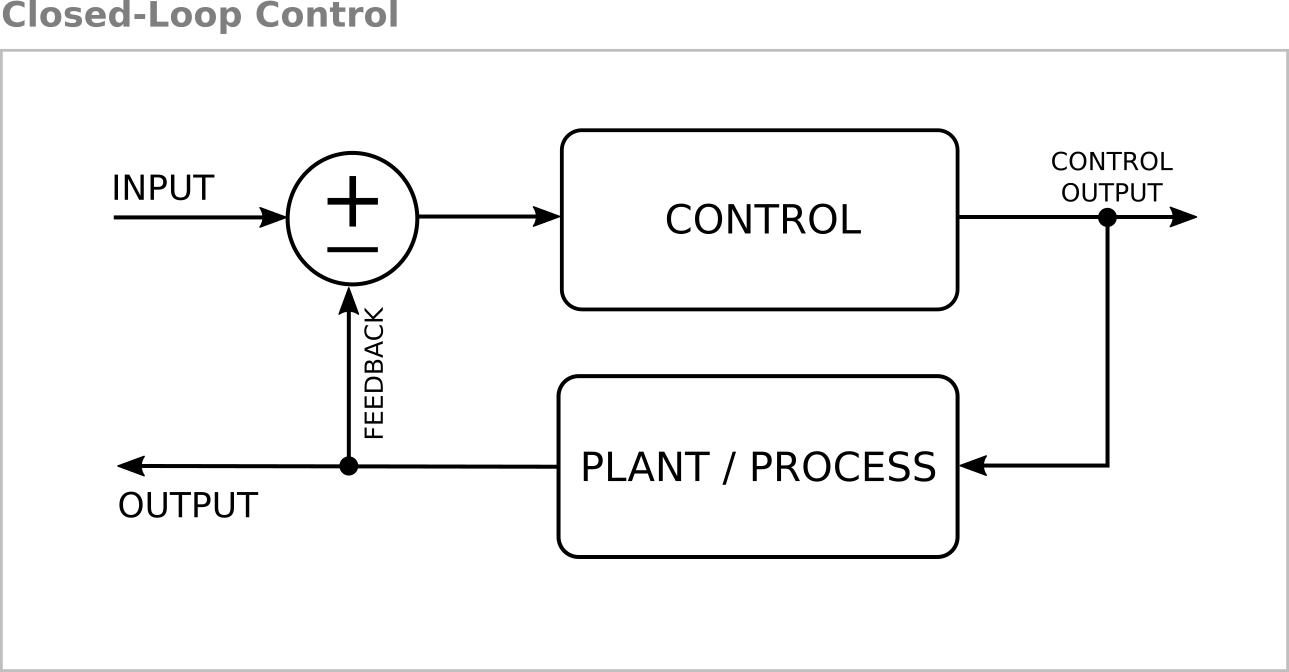
\includegraphics[width=.8\textwidth]{control_block}
    %\parbox{.75\textwidth}{\caption{Basic closed-loop control system. The output from the control block is fed into the physical ``plant'' and the generated output is compared against the target input.}}
    \caption{Basic closed-loop control system.}
    \label{control_block}
\end{figure}

\begin{description}
    \item [Input/Setpoint:] The input to a control system represents some parameter of the desired output. This \textit{setpoint} is compared against the current output state. 
    \item [Plant/Process:] The \textit{plant} of a system represents the external device under the command of the control system. The plant generates the observable output.
    \item [Feedback:] In a closed-loop system the output is compared against the input and the system's error is calculated. This error is often either the combination of the output and input (positive feedback) or the difference between them (negative feedback).
    \item [Control:] The control system adjusts its output (input to the plant) in order to minimize the system error. 
\end{description}

\subsection{PID Control Systems}
The acronym PID represents the three mathematical relations used within the control system; and stand for proportional, integral, and derivative. PID controllers are commonly used in industrial systems because they offer rapid error correction, good stability and can be tuned to react properly to the unique characteristics of a specific system.

The overall equation of a PID control system can be modeled by the following equation, where $c(t)$ represents the output control, and $e(t)$ the input error. 

    \begin{equation*}
    c(t) = K_{p}e(t) + K_{i}\int_{0}^{t}e(\tau)d\tau + K_{d}\frac{de(t)}{dt}
    \end{equation*} 

The outputs of each portion (proportional, integral, derivative) are combined to form the control signal fed to the system plant. The PID controller is tuned by adjusting scaling coefficients for each of these. Each of the three portions can be used in isolation to make simpler control systems. The following sections describe the effect each of the mathematical relationships has on the control signal depending on the input error. 

%A PID controller continuously calculates the system error from the input setpoint and feedback from the plant/process output. The controller generates a correction signal by combining values  
%Brief history and definition of PID control 

\begin{figure}[tb]
    \centering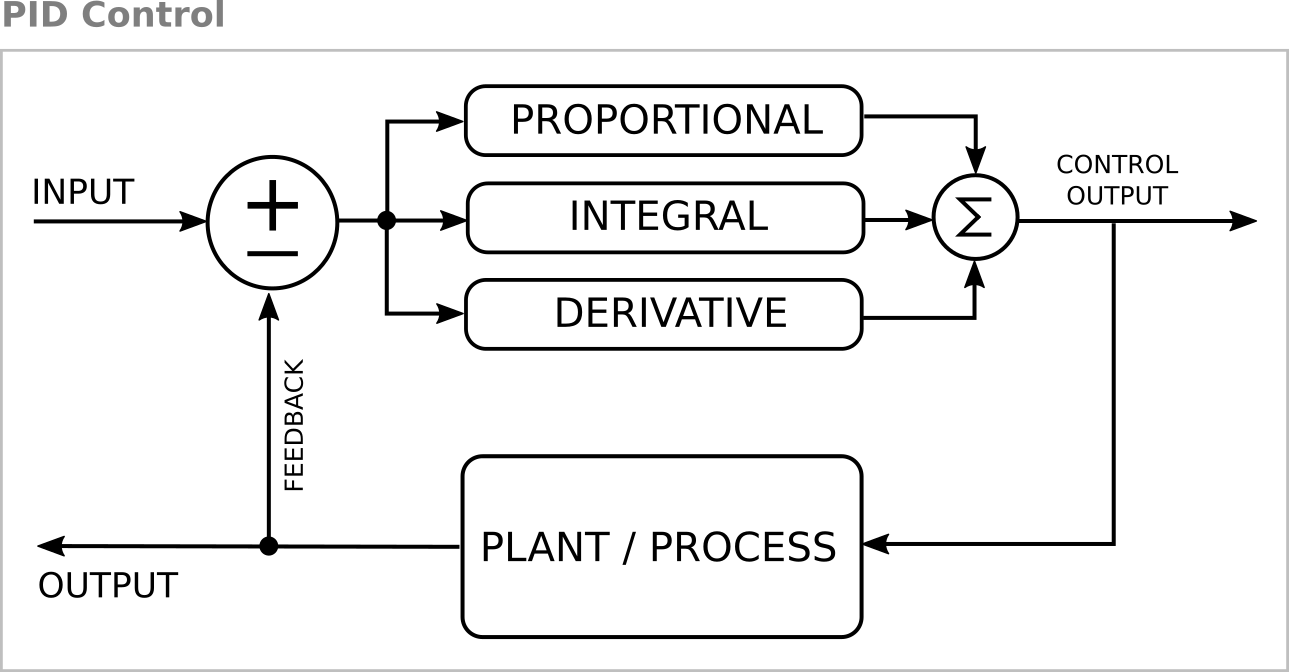
\includegraphics[width=.8\textwidth]{pid_block}
    \caption{PID Control System Block Diagram.}
    \label{pid_block}
\end{figure}

\subsubsection{Proportional}
The proportional control factor represents the following relationship between the output control signal and the input error:
\begin{equation*}
 c(t) = K_{p}e(t) 
\end{equation*} 

The constant $K_{p}$ is the proportional scaling coefficient and determines the strength of the action taken to correct the error signal. Proportional feedback applies an output signal proportional to the error, essentially scaling the error by $K_{p}$.
Proportional control provides rapid correction when the error signal is large, but loses effectiveness as the plant output nears the setpoint. Additionally, proportional control has the limitation that can not not adjust if the error persists through the initial action. 

\subsubsection{Integral}
Integral control grows proportionally to the integral of the error signal, and represents the following portion of the PID equation:

\begin{equation*}
c(t) = K_{i}\int_{0}^{t}e(\tau)d\tau
\end{equation*} 

Integral control begins with a small value regardless of the error's magnitude, but increases with the duration of the error. This means that even small errors will eventually build into large correction factors. This offers an advantage over proportional control as an integral based system will continually adjust until the error is corrected. The growth of the accumulated error is scaled by the integral scaling coefficient $ K_{i}$.

Because these systems are based on the integral of the error signal, they have the disadvantages of beginning slowly, and overshooting the target setpoint. This overshoot is caused by the need for an equal amount of negative error to be accumulated to return the integral's value back to zero. This phenomenon is called ``wind-up'' and is managed in most systems by setting a maximum value that the integral is allowed to accumulate. 

\subsubsection{Derivative}
The final portion of the PID controller is derivative control, representing the last portion of the system equation:

\begin{equation*}
c(t) = K_{d}\frac{de(t)}{dt}
\end{equation*} 

A derivative controller reacts to the rate of change in the output of the system. Typically derivative effects are used to minimize overshoot oscillations caused by integral control. However, they also respond rapidly to unexpected changes in the output of the system. The reactive strength of a derivative controller depends on it's scaling factor $K_{d}$.

The major drawback for derivative controlled systems is that they can amplify minor errors or oscillate in systems with natural fluctuations. Derivative systems are more difficult to tune properly, and depending on the process many systems use only proportional and integral control. 

\setSectionType{Review}
\section{Modeling DC Motors}

DC motors when operating steady-state appear mostly as a series resistive-inductive loop with a voltage drop dependent on the current angular velocity. This voltage drop is due to the back-electromotive force or EMF which is generated from the motion of the motor armature relative to the windings. Figure \ref{motor_sys} shows a model of a simple DC motor system. 

\subsection{Equations Modeling a Motor System}

There are a number of basic equations that model aspects of a motor system. In this lab we will be primarily concerned with only first-order effects, many of the complex parameters are either simplified or removed. 

\begin{figure}[tb]
    \centering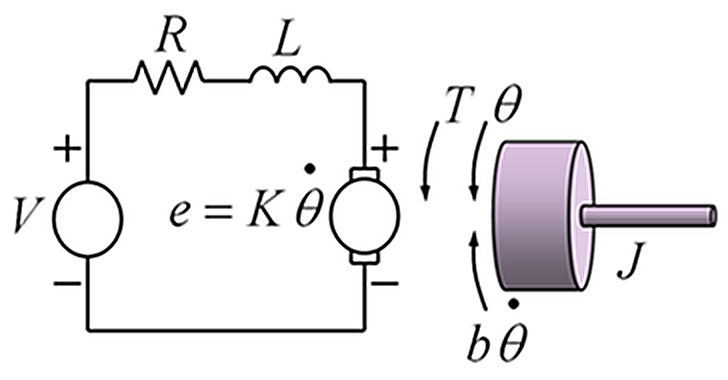
\includegraphics[width=.75\textwidth]{motor}
    \caption{Variables and constants in a motor system.}
    \label{motor_sys}
\end{figure}

The following equations use the following terminology:
\begin{itemize}
    \item $V$ -- DC drive voltage
    \item $R$ -- Motor winding resistance
    \item $L$ -- Motor winding inductance 
    \item $i$ -- Motor current 
    \item $\theta$ -- Angular position
    \item $\dot{\theta}$ -- Angular velocity (rotational speed)
    \item $\ddot{\theta}$ -- Angular acceleration
    \item $T$ -- Motor Torque
    \item $f$ -- System friction
    \item $K$ -- Torque constant
    \item $e$ -- Electromotive force
    \item $J$ -- Moment of inertia
    \item $t$ -- Time, ($s$ is used once in Laplace domain) 
\end{itemize}

\subsubsection{Torque Equation}
\begin{equation}
T(t) = Ki(t) = J\frac{d\dot{\theta}}{dt}=J\ddot{\theta}(t) 
\end{equation}

\subsubsection{Electromotive Force}
\begin{equation}
e(t) = K\dot{\theta}(t)
\end{equation}

\subsubsection{Kirchhoff's Law}
\begin{equation}
v(t) = Ri(t) + e = Ri(t) + K\dot{\theta}(t) = \frac{RJ}{K}\ddot{\theta}(t)+K\dot{\theta}(t)
\end{equation}

\subsubsection{1st-Order Transfer Function}
\begin{equation}
\frac{\dot{\theta}(s)}{v(s)} = \frac{1}{\frac{RJ}{K}s+K}
\end{equation}

% Section about deriving a motor transfer function

% Section about using Matlab/Simulink
   % probably just describe what they are and link to the resources
   
\subsection{Deriving the Transfer Functions}
When modeling any system the first step is to derive the characteristic transfer function. This equation represents the modeled system and supposedly responds in a mathematically accurate way when set with parameter values. Within this lab you are going to derive the transfer function of a theoretical DC motor and use simple integer values for many of its parameters. 

The typical form of a transfer function of a DC motor is the angular velocity (output) divided by the input voltage $\frac{\dot{\theta}(s)}{v(s)}$. Using this function gives a reasonable estimate of motor velocity for a specific input voltage. However, as shown in the lab exercises, other coefficients such as friction will play a large role in the output of the system. 

To derive the 1st-order transfer function, follow these steps. Your goal is to combine the torque and Kirchoff's equations together and then simplify using Laplace transformations. 
\begin{enumerate}
    \item Start with the mechanical torque equation. 
    \item Solve for the motor current $i$ by rearranging the torque equation. 
    \item Replace the torque $T$ term with its acceleration form in the rearranged current equation. (acceleration form listed above)  
    \item Replace the current $i$ term in Kirchoff's law with the rearranged current equation.
    \item Replace the electromotive force $e$ term in Kirchoff's law with its velocity and torque constant form. 
    \item Perform a Laplace transform of the modified equation, using an identity to convert the acceleration term into velocity. 
    \item Isolate the velocity term on the left-hand side with the voltage as the denominator
\end{enumerate}




\setSectionType{Exercise}
\section{Lab Assignment: Derivation of a DC Motor Transfer Function}
The following portions of the exercise create the ``plant'' or motor model used in the simulated control system. You will use your derived transfer functions within the Simulink model created in the second exercise. 
\begin{enumerate}
    \item Derive the first-order transfer function (velocity/voltage) of a DC motor without any friction and inductive effects. 
    \begin{itemize}
        \item You may wish to review class lecture 16 slides, the transfer function is shown there as well as this manual. You will need to show derivation work for credit! 
        \item You will need to use Laplace transformations to solve your first-order transfer function. 
        \item Your final equation should have the form: $\frac{\dot{\theta}(s)}{v(s)} = \,?$
    \end{itemize}
    \item Assuming the simple case where the torque constant \textit{K}, the moment of inertia \textit{J}, and the electrical resistance \textit{R}, all have a numerical value of 1, simulate the response of the function to a step of amplitude 1 using Matlab.
    \begin{itemize}
        \item The step function represents suddenly turning the motor on (providing voltage) when the motor was previously idle. 
        \item You will need to create a vector containing values representing the step function and pass it through the derived transfer function.
        \item The resulting output vector is the motor's velocity response.
    \end{itemize}
    \item Study and report the effects that changing the torque constant \textit{K}, moment of inertia \textit{J}, or electrical resistance \textit{R}, have on the motor's response to the step function.
    \item Derive the transfer function of a DC motor with friction. Note that the effect of friction can be modeled as an opposed torque of value $f\dot{\theta}$ (with \textit{f} the friction constant).
\end{enumerate}

\section{Lab Assignment: Simulating the Motor in Simulink}
Within this exercise you will convert your transfer function into a form that can be used within a Simulink model. You will use your model to experiment with changing the basic motor parameters under the influence of friction.
%\ddot{\theta}

\begin{enumerate}
    \item In order to use your transfer function within Simulink, you will need to rewrite to represent only the velocity. 
    \begin{itemize}
        \item Your original transfer function was in the form $\frac{\dot{\theta}(s)}{v(s)} = \,?$, you will need to convert it into $\dot{\theta}(s) = \frac{1}{s}*\,?$
        \item You will want to isolate the Laplace ``$s$'' term from the rest of the equation. This is because Simulink represents integration as a discrete ``$\frac{1}{s}$'' block. 
    \end{itemize}
    \item Create a Simulink subsystem model of the transfer function you derived. It should take the coefficients for the moment of inertia, friction, torque constant and voltage.
    \begin{itemize}
        \item See Figures \ref{subsystem} and \ref{subsystem_detail} for examples of what the interface and contents of the subsystem should resemble. (Figure \ref{subsystem_detail} doesn't represent an actual transfer function. \textbf{Don't try to use it!})
        \item Assume that the motor resistance is 1 to simplify the system. ($R=1$)
        \item The following tutorial on subsystems may be helpful:\\ \href{http://www.mathworks.com/help/simulink/ug/creating-subsystems.html}{http://www.mathworks.com/help/simulink/ug/creating-subsystems.html}
     \end{itemize}
    \item Simulate the system using a step function of amplitude 1 for the voltage; with values for the torque constant \textit{K}, and moment of inertia \textit{J} set to 1. 
    \begin{itemize}
        \item Simulate the model using different values for the friction parameter.
        \item The results should be similar to the second portion of the first exercise when the friction factor is zero. What happens if when the friction factor increases?
    \end{itemize}
    \item Perform a simulation with a step function controlling the friction parameter. (so it changes in the middle of the simulation) What happens, and why would friction dynamically change in a physical system? 
\end{enumerate}

\section{Lab Assignment: Designing a PI Controller in Simulink}
This exercise simulates portions of a PI (proportional \& integral) control system within the Simulink modeling framework. After completing this portion, you should understand the basic operation and be able to tune the modeled system for reasonable performance. 

\begin{enumerate}
    \item Implement a feedback control using only the proportional term. 
    \begin{itemize}
        \item Add a saturation block/module on the output of the control system. Set this limiter to allow a maximum value of 6. This approximates reasonable limitations of your drive hardware which can't increase the output voltage past what is supplied.  
        \item Study and comment the response of the system.
    \end{itemize}
    \item Improve the feedback control loop by adding an integral term. 
    \begin{itemize}
        \item Study and comment on the response of the system.
        \item You may need to scale the integral and proportional terms to prevent the system from oscillating.
    \end{itemize}
    
    
\end{enumerate}




\begin{figure}[tb]
    \centering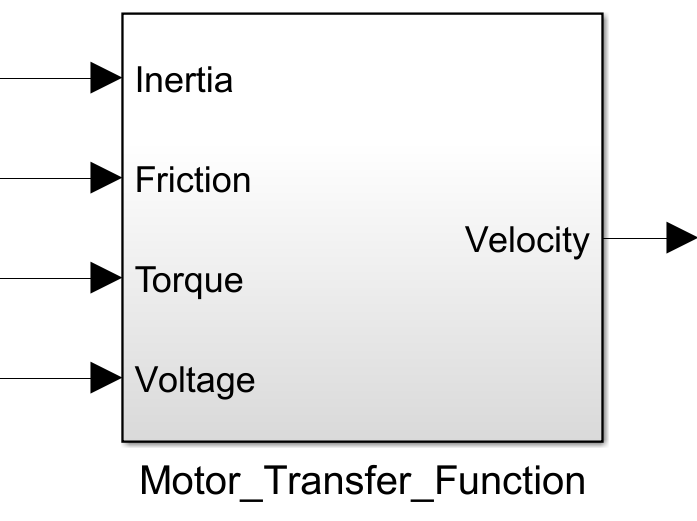
\includegraphics[width=.5\textwidth]{subsystem}
    \caption{Example motor transfer function subsystem interface.}
    \label{subsystem}
\end{figure}


%% Full-width figure
\begin{figure}[b]
    \begin{center}
        \hspace*{-3.4cm}
        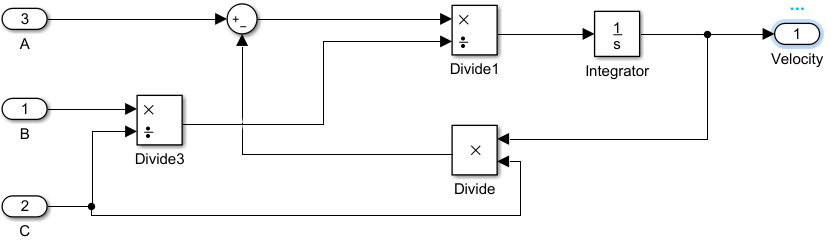
\includegraphics[width=0.8\paperwidth]{subsystem_detail}
        \caption{Example motor transfer function subsystem contents.}
        \label{subsystem_detail}
    \end{center}
\end{figure}


\end{document}

%% Full-width figure
%\begin{figure}[]
%    \begin{center}
%        \hspace*{-3.4cm}
%        
\includegraphics[width=0.8\paperwidth]{placeholder}
%        \caption{Fundamental wave shapes.}
%        \label{waves}
%    \end{center}
%\end{figure}